%% Problema: deve essere grassetto nella ToC e nel titolo del capitolo, ma non grassetto nell'header.
\chapter{Signal event selection}
\label{cap:event_selection}

\section{Prefiltering}
\label{sec:prefilter}
I grafici necessari probabilmente ha senso metterli qui. Magari puoi cambiare il nome in "prefiltering and data characteristics".

\begin{figure}[t]
	\centering
	\begin{subfigure}{.45\textwidth}
		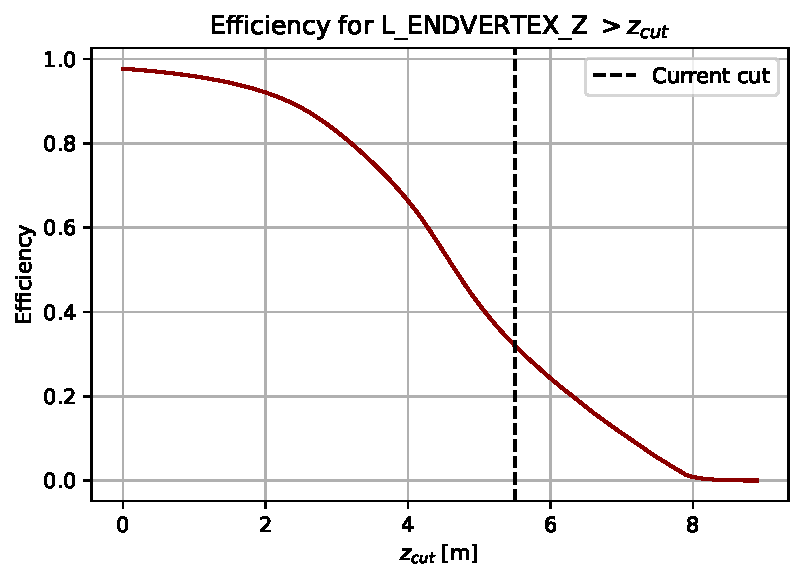
\includegraphics[width=\textwidth]{graphics/04-event_selection/LEVz_left.pdf}
		\caption{}
	\end{subfigure}
	\begin{subfigure}{.45\textwidth}
		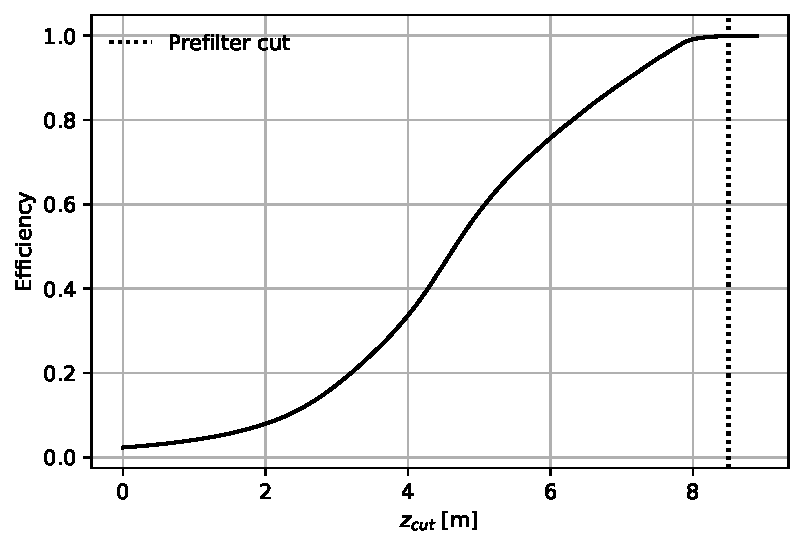
\includegraphics[width=\textwidth]{graphics/04-event_selection/LEVz_right.pdf}
		\caption{}
	\end{subfigure}
	\caption[A and b.]{Boh...}
\end{figure}

\begin{figure}[t]
	\centering
	\begin{subfigure}{.45\textwidth}
		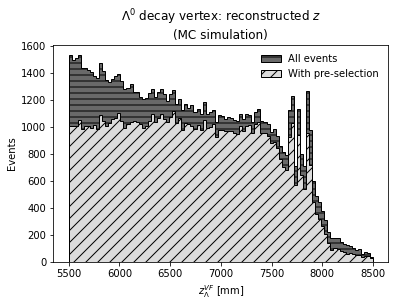
\includegraphics[width=\textwidth]{graphics/04-event_selection/Lambda_endvertex_z.png}
		\caption{}
	\end{subfigure}
	\begin{subfigure}{.45\textwidth}
		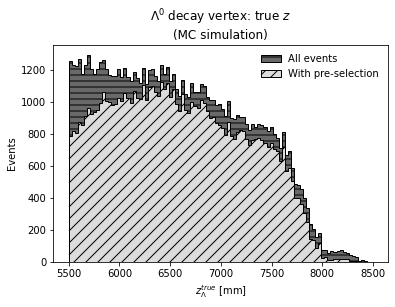
\includegraphics[width=\textwidth]{graphics/04-event_selection/Lambda_endvertex_z_true.png}
		\caption{}
	\end{subfigure}
	\caption[Distribution of reconstructed and true $z_\Lambda^\text{vtx}$ in simulated $\Lambda_b^0$ signal events.]{Distribution of reconstructed (\textit{left}) and true (\textit{right}) $z_\Lambda^\text{vtx}$ in simulated $\Lambda_b^0$ signal events, without (\textit{dark grey}) and with (\textit{light grey}) prefiltering.}
\end{figure}

\begin{figure}[t]
	\centering
	\begin{subfigure}{.45\textwidth}
		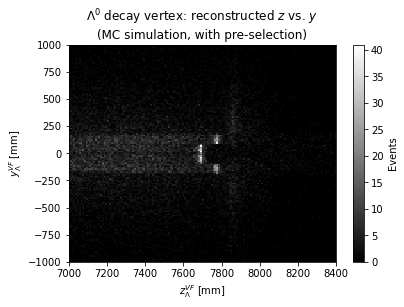
\includegraphics[width=\textwidth]{graphics/04-event_selection/Lambda_endvertex_z_vs_x.png}
		\caption{}
	\end{subfigure}
	\begin{subfigure}{.45\textwidth}
		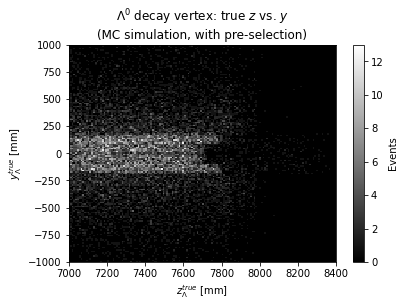
\includegraphics[width=\textwidth]{graphics/04-event_selection/Lambda_endvertex_z_vs_x_true.png}
		\caption{}
	\end{subfigure}
	\caption[Event distribution of simulated $\Lambda_b^0$ signal events as a function of reconstructed and true $x_\Lambda^\text{vtx}$ and $z_\Lambda^\text{vtx}$.]{Event distribution of simulated $\Lambda_b^0$ signal events as a function of reconstructed (\textit{left}) and true (\textit{right}) $x_\Lambda^\text{vtx}$ and $z_\Lambda^\text{vtx}$.}
\end{figure}

Confronto con Figure \ref{fig:2:t_station_top}.

\subsection{Bias in \texorpdfstring{\lz}{Lambda} decay vertex}
\label{sec:lambda_endvertex_bias}
\begin{figure}[t]
	\centering
	\begin{subfigure}{.45\textwidth}
		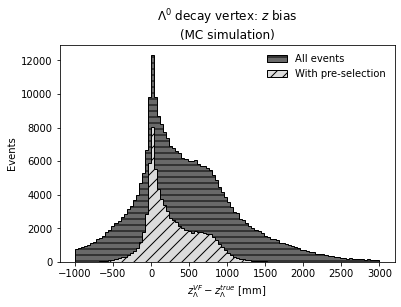
\includegraphics[width=\textwidth]{graphics/04-event_selection/LEVz_MC_true-residuals.png}
		\caption{}
	\end{subfigure}
	\begin{subfigure}{.45\textwidth}
		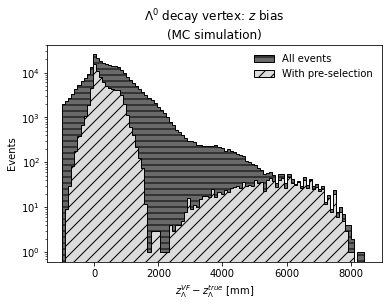
\includegraphics[width=\textwidth]{graphics/04-event_selection/LEVz_MC_true-residuals_log.png}
		\caption{}
	\end{subfigure}
	\caption{Aboh.}
\end{figure}

\begin{figure}[t]
	\centering
	\begin{subfigure}{.45\textwidth}
		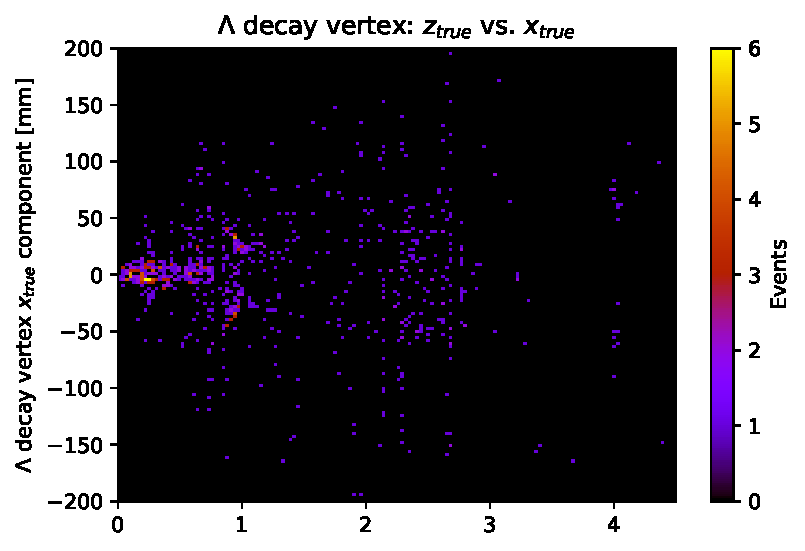
\includegraphics[width=\textwidth]{graphics/04-event_selection/LEVz_MC_ztrue-vs-xtrue.pdf}
		\caption{}
	\end{subfigure}
	\begin{subfigure}{.45\textwidth}
		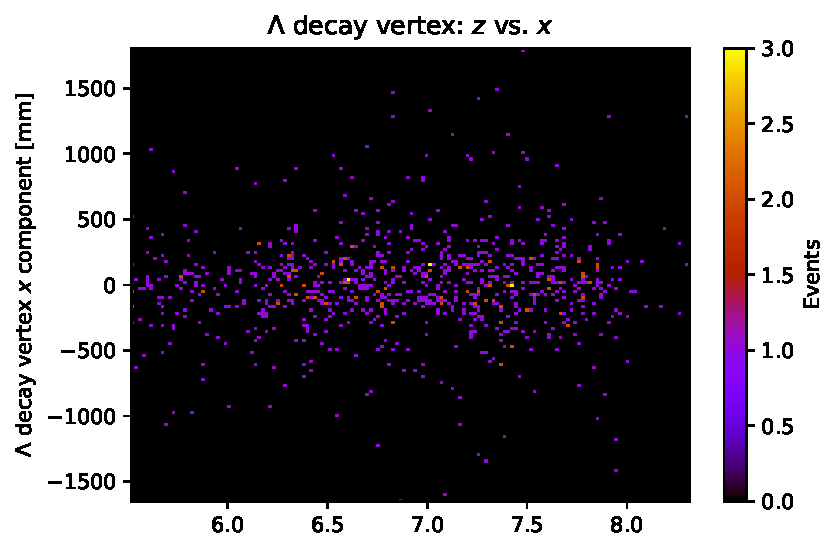
\includegraphics[width=\textwidth]{graphics/04-event_selection/LEVz_MC_z-vs-x.pdf}
		\caption{}
	\end{subfigure}
	\caption[A and b.]{Boh...}
\end{figure}


Qui devi menzionare l'orizzontalità, perché vi faccio riferimento nel Cap. 3. Devi dire che c'è il problema con grafico.

\section{HBDT classifier}
\label{sec:HBDT}

\subsection{Training data}

\begin{figure}[t]
	\centering
	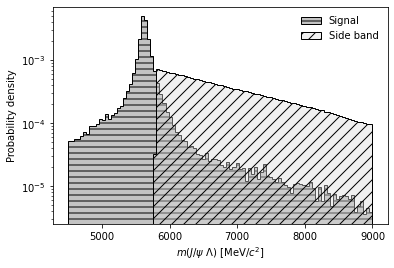
\includegraphics[width=.6\textwidth]{graphics/04-event_selection/hbdt_signal_sidebands.png}
	\caption{A.}
	\label{fig:4:HBDT_training_data}
\end{figure}

\subsection{Hyperparameter optimization and performance test}

\subsection{Threshold optimization}

\section{Physical background veto}
\label{sec:B0_veto}

\section{Performance on data}
Gli invariant mass fits, essenzialmente.